\documentclass[11pt,a4paper]{article}

% ============================================================
% PACKAGES
% ============================================================
\usepackage[margin=2.2cm]{geometry}
\usepackage{times}
\usepackage[T1]{fontenc}
\usepackage{titlesec}
\usepackage{enumitem}
\usepackage{booktabs}
\usepackage{array}
\usepackage{longtable}
\usepackage{xcolor}
\usepackage{colortbl}
\usepackage{tabularx}
\usepackage{graphicx}
\usepackage{amsmath,amssymb}
\usepackage{siunitx}
\usepackage{fancyhdr}
\usepackage{caption}
\usepackage{float}
\usepackage[ruled,vlined,linesnumbered]{algorithm2e}
\usepackage{tikz}
\usetikzlibrary{shapes.geometric, arrows.meta, positioning, calc, fit, backgrounds}
\usepackage{hyperref}

% ============================================================
% COLOURS (team house style)
% ============================================================
\definecolor{isrogreen}{RGB}{0,90,60}
\definecolor{isroorange}{RGB}{230,110,20}
\definecolor{tblhead}{RGB}{0,90,60}
\definecolor{lightgray}{RGB}{240,240,240}
\definecolor{goodgreen}{RGB}{20,120,50}
\definecolor{warnamber}{RGB}{190,120,0}
\definecolor{badred}{RGB}{170,30,30}
\definecolor{phhome}{RGB}{42,120,214}
\definecolor{phloit}{RGB}{235,104,52}
\definecolor{phfin}{RGB}{27,175,122}

\titleformat{\section}{\normalfont\Large\bfseries\color{isrogreen}}{\thesection}{1em}{}
\titleformat{\subsection}{\normalfont\large\bfseries\color{isroorange}}{\thesubsection}{1em}{}
\titleformat{\subsubsection}{\normalfont\bfseries}{\thesubsubsection}{1em}{}

\pagestyle{fancy}
\fancyhf{}
\renewcommand{\headrulewidth}{0.6pt}
\renewcommand{\footrulewidth}{0.4pt}
\lhead{\small CU Jammu Astro: Autonomous Parafoil Targeted Landing}
\rhead{\small ISRO / IN-SPACe CanSat 2026}
\lfoot{\small Guidance, Firmware and Verification}
\rfoot{\small \thepage}
\setlength{\headheight}{14pt}

\hypersetup{colorlinks=true, linkcolor=isrogreen, urlcolor=isroorange, citecolor=isrogreen,
  pdftitle={Autonomous Parafoil Targeted Landing: Guidance, Firmware and Verification},
  pdfauthor={CU Jammu Astro CanSat Team}}

\setlist[itemize]{leftmargin=1.4em}
\setlist[enumerate]{leftmargin=1.6em}
\newcolumntype{Y}{>{\raggedright\arraybackslash}X}
\newcommand{\good}[1]{\textcolor{goodgreen}{\textbf{#1}}}
\newcommand{\warn}[1]{\textcolor{warnamber}{\textbf{#1}}}
\newcommand{\bad}[1]{\textcolor{badred}{\textbf{#1}}}
\newcommand{\hdr}[1]{\textcolor{white}{\textbf{#1}}}
\newcommand{\code}[1]{\texttt{#1}}
\newcommand{\vect}[1]{\mathbf{#1}}
\newcommand{\wrap}{\operatorname{wrap}}
\newcommand{\sat}{\operatorname{sat}}
\sisetup{per-mode=symbol}
\captionsetup{font=small, labelfont={bf,color=isrogreen}}

\begin{document}

% ============================================================
% TITLE PAGE
% ============================================================
\begin{titlepage}
\centering
\vspace*{1.2cm}
{\Huge\bfseries\color{isrogreen} Autonomous Parafoil}\\[0.3cm]
{\Huge\bfseries\color{isrogreen} Targeted Landing}\\[0.6cm]
{\LARGE\bfseries\color{isroorange} Guidance Algorithm, Flight Firmware\\[0.15cm] and Verification Report}\\[1.4cm]

{\large Energy-managed guidance for a 1\,kg CanSat under a steerable\\
single-skin parafoil, with an 80\,m landing-accuracy requirement}\\[1.6cm]

\begin{tabular}{ll}
\textbf{Team:} & CU Jammu Astro, CanSat Team 039 \\
\textbf{Programme:} & ISRO / IN-SPACe CanSat India Student Competition 2026 \\
\textbf{Subsystem:} & Recovery, Guidance and Flight Software \\
\textbf{Flight computer:} & Teensy 4.1 (ARM Cortex-M7, 600\,MHz) \\
\textbf{Requirement:} & Touchdown within \SI{80}{\meter} of the target coordinate \\
\textbf{Status:} & Bench and ground tests passed; not yet drop-tested \\
\textbf{Date:} & 5 October 2026 \\
\end{tabular}

\vspace{1.4cm}
\rule{0.6\textwidth}{0.4pt}

\vspace{0.5cm}
{\normalsize\itshape
This report documents the complete guided-landing system as built: the
problem analysis, every estimator and control law with its mathematics, the
flight-state machine, the firmware implementation, the Monte-Carlo
verification of the exact flight code, and the hardware bench results to
date. It states plainly what has been verified and what has not.}

\vfill
{\small Firmware package: \code{Parafoil\_Guided\_Landing/} \quad
(\code{Parafoil\_Guided\_Landing.ino}, \code{ParafoilGuidance.h},
\code{ResumeRecord.h}, \code{host\_sim/monte\_carlo.cpp})}
\end{titlepage}

\tableofcontents
\newpage

% ============================================================
\section{Executive Summary}
% ============================================================

The CanSat descends under a drogue to \SI{500}{\meter} above ground, then
releases a steerable single-skin parafoil. The task is to land within
\SI{80}{\meter} of a target coordinate.

The earlier controller pointed the canopy at the target and centred the
servos inside a \SI{35}{\meter} ``capture'' circle. A parafoil cannot stop or
slow down; it only glides. Pointing at the target makes it arrive with height
to spare and land wherever the leftover glide takes it. The team's own
simulation of that logic produced a \SI{617.7}{\meter} miss.

The new system manages \emph{energy}, not just direction:

\begin{enumerate}
  \item It computes a \textbf{virtual target}: the point in the moving air
        that the wind will carry onto the real target exactly at touchdown.
        This turns the windy problem into a still-air problem.
  \item It compares the glide still available with the distance to that
        point. The difference is \textbf{excess energy}, measured in metres
        of air path.
  \item It flies four phases: \textbf{HOMING} toward the virtual target,
        \textbf{LOITER} in a \SI{50}{\meter} orbit to burn excess height,
        \textbf{FINAL} approach with S-turns to burn the last metres, and
        \textbf{TERMINAL} wings-level flight below \SI{8}{\meter}.
  \item Wind and airspeed are \textbf{measured in flight} from GPS ground
        velocity during turns; sink rate is measured by the barometer.
        No canopy parameter needs to be known in advance.
\end{enumerate}

\noindent\textbf{Verification.} The guidance core is a single C++ header
compiled identically by the Teensy firmware and by a PC Monte-Carlo
harness. Over 3000 randomised flights (canopy, wind, sensors, GPS dropouts
all varied):

\begin{center}
\renewcommand{\arraystretch}{1.25}
\begin{tabular}{lccc}
\toprule
\textbf{Flight class} & \textbf{Flights} & \textbf{Within 80\,m} & \textbf{Median miss} \\
\midrule
All physically reachable targets & 2684 & \good{98.3\,\%} & \SI{14}{\meter} \\
Reach margin above \SI{150}{\meter} & 2451 & \good{99.8\,\%} & \SI{13.9}{\meter} (95th pct.\ \SI{34}{\meter}) \\
Old point-at-target logic, same reachable flights & 2684 & 97.2\,\% & \SI{30}{\meter} \\
\bottomrule
\end{tabular}
\end{center}

\noindent\textbf{Hardware status.} All sensors, both steering servos, the
GPS at \SI{5}{\hertz}, the in-firmware simulated flight (\SI{13.9}{\meter}
miss on real servos) and an outdoor walking test have passed. SD logging and
the hardware watchdog are the remaining bench items. \textbf{No drop test
has been flown yet}; every canopy number used so far is a modelling range,
not a measurement (Section~\ref{sec:limits}).

% ============================================================
\section{Problem Definition}
% ============================================================

\subsection{Mission profile}
From the CanSat CDR: ejection at apogee (about \SI{1000}{\meter} AGL), a
conical drogue to stabilise the payload at roughly \SI{20}{\meter\per\second},
servo-actuated release of the parafoil at \SI{500}{\meter} AGL, an
``8-second patience'' window for pendulum damping, then guided descent.
Steering is by pulling the left or right trailing-edge brake line through a
continuous-rotation ST-3009 servo and spool.

\subsection{Why pointing at the target fails}
Let $h$ be height above the target ground, $V_z$ the sink rate and $V_a$ the
airspeed. In still air, the horizontal distance the canopy can still fly is
\begin{equation}
  L = V_a\, t_{go}, \qquad t_{go} = \frac{h}{V_z}.
\end{equation}
With $V_a = \SI{6}{\meter\per\second}$ and $V_z = \SI{2.5}{\meter\per\second}$,
$L \approx \SI{1200}{\meter}$ from \SI{500}{\meter}. If the target is
\SI{400}{\meter} away, flying straight at it leaves about \SI{800}{\meter}
of glide unused on arrival. A ``capture'' rule that stops steering at that
point lets the canopy glide straight on and land hundreds of metres beyond.
Accuracy therefore depends on \emph{using up the right amount of glide at the
right place}, which is an energy-management problem.

\subsection{Reachability}
Wind $\vect W$ moves the whole air mass. Over the remaining time the canopy
drifts by $\vect W t_{go}$, and it can additionally cover any displacement of
length up to $V_a t_{go}$ relative to the air. A target at the origin is
reachable from position $\vect p$ only if
\begin{equation}
  \bigl\lVert -\vect p - \vect W\, t_{go} \bigr\rVert \le V_a\, t_{go}.
  \label{eq:reach}
\end{equation}
No guidance law can beat this bound. If the deployment point is outside the
reachable region, the best possible result is the minimum-distance landing,
and the 80\,m requirement cannot be met regardless of software.

% ============================================================
\section{System Architecture}
% ============================================================

\subsection{Hardware used for the guided-landing system}
\begin{center}
\small
\renewcommand{\arraystretch}{1.2}
\begin{tabularx}{\linewidth}{p{3.3cm}p{3.6cm}Y}
\toprule
\rowcolor{tblhead}\hdr{Function} & \hdr{Device} & \hdr{Interface and notes} \\
\midrule
Flight computer & Teensy 4.1 & 600\,MHz Cortex-M7 with double-precision FPU \\
GNSS & Foxeer M10Q-180 (u-blox M10) & UART Serial3, \SI{38400}{baud}; GPS TX $\to$ pin 15 (RX3), GPS RX $\to$ pin 14 (TX3); VCC 5\,V \\
Barometer & Bosch BMP581 & I\textsuperscript{2}C 0x46/0x47, register-level driver \\
IMU & LSM6DSO32 & I\textsuperscript{2}C 0x6A; yaw-rate source \\
Magnetometer & QMC5883 & I\textsuperscript{2}C 0x0D; heading fallback only \\
Steering servos & 2 $\times$ Feetech ST-3009 & Serial1 half-duplex, \SI{1}{Mbps}, IDs 1 (left) and 2 (right), neutral 2048 \\
Deployment servo & SG90 & PWM pin 8; \SI{140}{\degree} locked, \SI{180}{\degree} released \\
Data logger & Teensy built-in microSD & \code{FLTnnn.CSV} at \SI{10}{\hertz} \\
\bottomrule
\end{tabularx}
\end{center}
\noindent The I\textsuperscript{2}C bus is shared on SDA pin 18 and SCL pin 19 at
\SI{400}{\kilo\hertz}. Sensors run from the Teensy \SI{3.3}{\volt} rail; the
ST-3009 servos have their own supply (measured \SI{7.6}{\volt}) with a common
ground.

\subsection{Software structure}
\begin{figure}[H]
\centering
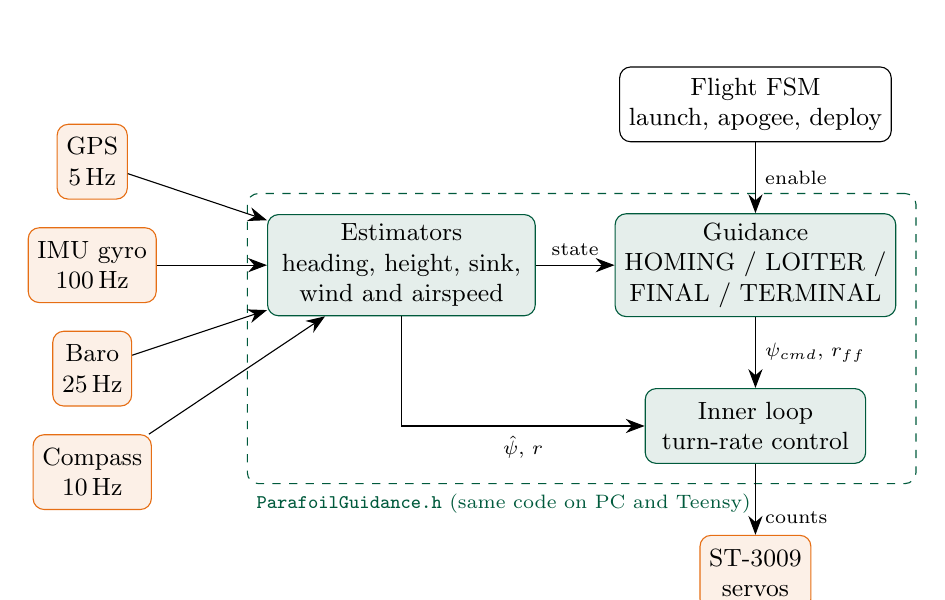
\begin{tikzpicture}[
  box/.style={draw, rounded corners, align=center, minimum height=0.95cm, font=\small, fill=white},
  core/.style={box, fill=isrogreen!10, draw=isrogreen},
  hw/.style={box, fill=isroorange!10, draw=isroorange},
  >={Stealth[length=2.4mm]}]
\node[hw] (gps) {GPS\\5\,Hz};
\node[hw, below=0.35cm of gps] (imu) {IMU gyro\\100\,Hz};
\node[hw, below=0.35cm of imu] (baro) {Baro\\25\,Hz};
\node[hw, below=0.35cm of baro] (mag) {Compass\\10\,Hz};
\node[core, right=1.4cm of imu, minimum width=3.4cm] (est) {Estimators\\heading, height, sink,\\wind and airspeed};
\node[core, right=1.0cm of est, minimum width=2.8cm] (gd) {Guidance\\HOMING / LOITER /\\FINAL / TERMINAL};
\node[core, below=0.9cm of gd, minimum width=2.8cm] (in) {Inner loop\\turn-rate control};
\node[hw, below=0.9cm of in] (srv) {ST-3009\\servos};
\node[box, above=0.9cm of gd, minimum width=2.8cm] (fsm) {Flight FSM\\launch, apogee, deploy};
\draw[->] (gps) -- (est); \draw[->] (imu) -- (est); \draw[->] (baro) -- (est); \draw[->] (mag) -- (est);
\draw[->] (est) -- node[above, font=\scriptsize]{state} (gd);
\draw[->] (gd) -- node[right, font=\scriptsize]{$\psi_{cmd}$, $r_{ff}$} (in);
\draw[->] (est.south) |- node[pos=0.75, below, font=\scriptsize]{$\hat\psi$, $r$} (in.west);
\draw[->] (in) -- node[pos=0.75, right, font=\scriptsize]{counts} (srv);
\draw[->] (fsm) -- node[right, font=\scriptsize]{enable} (gd);
\begin{scope}[on background layer]
\node[draw=isrogreen, dashed, rounded corners, inner sep=0.25cm, fit=(est)(gd)(in),
      label={[font=\scriptsize, text=isrogreen, anchor=north west]south west:{\code{ParafoilGuidance.h} (same code on PC and Teensy)}}] {};
\end{scope}
\end{tikzpicture}
\caption{Data flow. Everything inside the dashed box lives in
\code{ParafoilGuidance.h} as the class \code{FlightCore}. The \code{.ino}
handles hardware, the flight-state machine, commands and logging.}
\end{figure}

\begin{center}
\small
\renewcommand{\arraystretch}{1.2}
\begin{tabularx}{\linewidth}{p{5.6cm}Y}
\toprule
\rowcolor{tblhead}\hdr{File} & \hdr{Contents} \\
\midrule
\code{ParafoilGuidance.h} & Pure C++, no Arduino dependency: geodesy, filters, wind estimator, guidance, inner loop, \code{FlightCore}, simulation model. \\
\code{Parafoil\_Guided\_Landing.ino} & Sensor drivers, servo bus, flight-state machine, EEPROM resume, SD log, USB command interface, SIM and WALK bench modes. \\
\code{ResumeRecord.h} & EEPROM record for in-flight reset recovery (separate header so the Arduino prototype generator does not break it). \\
\code{host\_sim/monte\_carlo.cpp} & PC test harness: randomised flights through the same \code{FlightCore}. \\
\bottomrule
\end{tabularx}
\end{center}

% ============================================================
\section{Conventions and Coordinate Frames}
% ============================================================

\begin{itemize}
  \item \textbf{Local frame:} North and East in metres, origin at the target.
  \item \textbf{Heading:} degrees; $0^\circ$ is North, angles increase
        clockwise, so $90^\circ$ is East. $\wrap_{180}(\cdot)$ maps an angle to
        $(-180^\circ, 180^\circ]$.
  \item \textbf{Steering demand $u$:} servo counts, \textbf{positive = turn
        right}. Saturated at $\pm 450$ counts (about $\pm\SI{40}{\degree}$ of
        servo rotation).
  \item \textbf{Height $h$:} metres above the target's ground level.
        \textbf{Sink rate $V_z > 0$} means descending.
  \item \textbf{Wind $\vect W$:} the direction the air is moving \emph{to}.
\end{itemize}

\subsection{Latitude and longitude to local metres}
An equirectangular projection about the target $(\varphi_0, \lambda_0)$:
\begin{align}
  m_\varphi &= 111132.92 - 559.82\cos 2\varphi_0 + 1.175\cos 4\varphi_0 \quad [\si{\meter\per\degree}],\\
  m_\lambda &= 111412.84\cos\varphi_0 - 93.5\cos 3\varphi_0 \quad [\si{\meter\per\degree}],\\
  p_N &= (\varphi - \varphi_0)\, m_\varphi, \qquad p_E = (\lambda - \lambda_0)\, m_\lambda .
\end{align}
The error is below 0.1\,\% over a few kilometres, far smaller than GPS noise.
Latitudes are kept in double precision.

% ============================================================
\section{State Estimation}
% ============================================================

\subsection{Barometric height}
At ARM the firmware averages 25 pressure samples to obtain the ground
reference $p_0$. Height above the target is
\begin{equation}
  h_{raw} = 44330\left[1 - \left(\frac{p}{p_0}\right)^{0.190295}\right] - \Delta h_{tgt} \quad [\si{\meter}],
\end{equation}
where $\Delta h_{tgt}$ (\code{TARGET\_ELEV\_OFFSET\_M}) is the target ground
height minus the ARM-point height. If the barometer fails, GPS altitude minus
its ARM value is used instead.

\paragraph{Alpha-beta filter.} Height $\hat h$ and vertical speed $\hat v$
(positive up) are smoothed at \SI{25}{\hertz} with $\alpha = 0.12$,
$\beta = 0.008$:
\begin{align}
  \hat h^- &= \hat h + \hat v\,\Delta t, \qquad e = h_{raw} - \hat h^-,\\
  \hat h &= \hat h^- + \alpha\, e, \qquad \hat v = \hat v + \frac{\beta}{\Delta t}\, e .
\end{align}
A gap $\Delta t > \SI{0.5}{\second}$ re-seeds the height and keeps the velocity.

\subsection{Sink rate}
Two first-order low-pass estimates with time constant $\tau_z = \SI{3}{\second}$
are kept:
\begin{itemize}
  \item $V_{z,all}$, updated continuously after canopy opening. Its history
        is discarded at $0.6\,T_{damp}$ (\SI{4.8}{\second}) to remove the
        opening shock.
  \item $V_{z,str}$, updated only after the yaw rate has stayed below
        \SI{6}{\degree\per\second} for \SI{2}{\second} (straight flight).
\end{itemize}
Guidance uses $V_{z,str}$ when available, otherwise $V_{z,all}$, otherwise
the default \SI{2.5}{\meter\per\second}. The straight-flight value is
preferred because the final approach is flown straight; turning increases
sink and would bias $t_{go}$.

\subsection{Heading: gyro and GPS complementary filter}
The guidance needs the \emph{air} heading $\psi$ (where the canopy points),
not the ground track. Between GPS fixes the estimate is propagated by the
bias-corrected gyro yaw rate $r$:
\begin{equation}
  \hat\psi \leftarrow \hat\psi + r\,\Delta t .
\end{equation}
At each GPS fix with ground speed $\ge \SI{1.5}{\meter\per\second}$ the air
velocity is formed by removing the wind estimate, and the heading is
corrected with gain $k_\psi = 0.3$:
\begin{align}
  \psi_{meas} &= \operatorname{atan2}\!\left(v_E - \hat W_E,\; v_N - \hat W_N\right) + r\,\tau_{lat}, \qquad \tau_{lat} = \SI{0.15}{\second},\\
  \hat\psi &\leftarrow \hat\psi + k_\psi\, \wrap_{180}\!\left(\psi_{meas} - \hat\psi\right).
\end{align}
The $r\,\tau_{lat}$ term compensates the GPS velocity delay during turns.
Before a wind estimate exists, $\hat{\vect W}=0$ and the filter tracks ground
course, which makes HOMING steer the ground track at the target. The QMC5883
compass is used only when no GPS heading has arrived for \SI{2}{\second}, with
gain 0.05, because it sits close to the servo motors and is not
tilt-compensated.

\subsection{Wind and airspeed from a circle fit}
\label{sec:wind}
In steady flight the ground velocity is
\begin{equation}
  \vect v_g = \vect W + V_a \begin{bmatrix}\cos\psi\\ \sin\psi\end{bmatrix}.
\end{equation}
As the canopy turns, the points $(v_N, v_E)$ lie on a circle whose
\textbf{centre is the wind} and whose \textbf{radius is the airspeed}. No
compass and no assumed airspeed are needed.

\paragraph{Algebraic least-squares fit.} The last $N \le 160$ GPS velocity
samples (\SI{32}{\second} at \SI{5}{\hertz}) are centred on their mean
$(\bar x, \bar y)$, giving $x_i, y_i$ with $\sum x_i = \sum y_i = 0$. Fitting
$x^2 + y^2 + a x + b y + c = 0$ by minimising
$\sum_i (z_i + a x_i + b y_i + c)^2$ with $z_i = x_i^2 + y_i^2$ gives the
normal equations
\begin{equation}
  \begin{bmatrix} S_{xx} & S_{xy}\\ S_{xy} & S_{yy}\end{bmatrix}
  \begin{bmatrix} a\\ b\end{bmatrix}
  = -\begin{bmatrix} S_{xz}\\ S_{yz}\end{bmatrix},
  \qquad c = -\frac{S_z}{N},
\end{equation}
with $S_{xx} = \sum x_i^2$, $S_{xz} = \sum x_i z_i$ and so on. Then
\begin{equation}
  \hat W_N = \bar x - \tfrac{a}{2}, \qquad \hat W_E = \bar y - \tfrac{b}{2}, \qquad
  \hat V_a = \sqrt{\tfrac{a^2 + b^2}{4} - c}.
\end{equation}

\paragraph{Acceptance tests.} A fit is rejected unless all of these hold:
\begin{itemize}
  \item at least 30 samples, and $\det > 10^{-3} S_{xx}S_{yy}$ (samples not on a line);
  \item \textbf{turn coverage measured by the gyro}: the gyro-integrated
        heading of the samples must occupy at least 9 of 12 \SI{30}{\degree}
        bins (\SI{270}{\degree}) for the first fit and 7 bins
        (\SI{210}{\degree}) afterwards, with at least 2 samples per bin;
  \item RMS radial residual $\le \SI{1.2}{\meter\per\second}$;
  \item $\SI{2.5}{} \le \hat V_a \le \SI{15}{\meter\per\second}$ and $\lVert\hat{\vect W}\rVert \le \SI{12}{\meter\per\second}$;
  \item after the first fit, $|\hat V_a - \hat V_a^{prev}| \le \SI{2.5}{\meter\per\second}$.
\end{itemize}
Accepted fits are blended with weight 0.3. The fit is attempted once per
second.

\paragraph{Why coverage comes from the gyro.} The first version measured
coverage as the angular spread of samples around the \emph{fitted} centre.
Monte-Carlo traces showed a short, noisy \SI{60}{\degree} arc being fitted by
a small wrong circle, which then looked well covered around its own centre
and produced a \SI{5}{\meter\per\second} wind in still air. Measuring coverage
from the independent gyro heading removed this failure.

\paragraph{Airspeed.} When the wind is known and the canopy has flown
straight for \SI{2}{\second}, $V_{a,str} = \lVert \vect v_g - \hat{\vect W}\rVert$
is low-pass filtered ($\tau = \SI{4}{\second}$). Priority:
$V_{a,str}$, then the fit radius, then the default \SI{6}{\meter\per\second}.

% ============================================================
\section{Guidance Law}
% ============================================================

\subsection{Virtual target}
Define the time to go and the remaining air path
\begin{equation}
  t_{go} = \frac{h}{V_z}, \qquad L = V_a\, t_{go},
\end{equation}
with $V_z$ clamped to $[0.8, 8]\,\si{\meter\per\second}$ and $V_a$ to
$[2.5, 15]\,\si{\meter\per\second}$. The \textbf{virtual target} is
\begin{equation}
  \vect p_{VT} = -\hat{\vect W}\, t_{go}.
\end{equation}

\paragraph{Property: the virtual target is fixed in the air mass.}
Since $\dot t_{go} = -1$ (one second of flight removes one second of time to
go),
\begin{equation}
  \frac{d\vect p_{VT}}{dt} = -\hat{\vect W}\,\dot t_{go} = \hat{\vect W}.
\end{equation}
The virtual target moves exactly with the wind, i.e.\ it is stationary
relative to the air, and it reaches the real target at $t_{go} = 0$.
Relative to the air, the canopy's motion is pure $V_a$ flight with no wind.
The whole windy problem therefore reduces to: \emph{reach the air-fixed
point $\vect p_{VT}$ using exactly $L$ metres of air path.}

\begin{figure}[H]
\centering
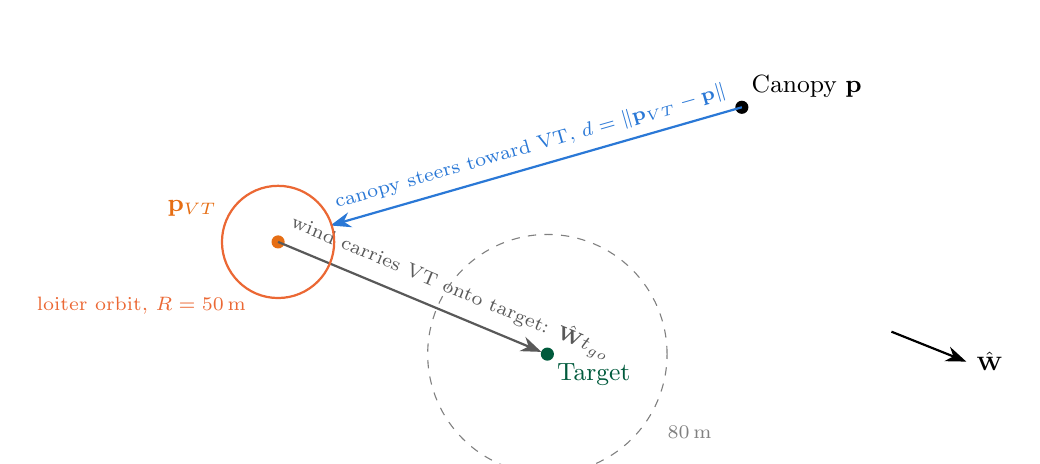
\begin{tikzpicture}[scale=0.95, >={Stealth[length=2.6mm]}]
\fill[isrogreen] (0,0) circle (2.5pt) node[below right, font=\small]{Target};
\draw[dashed, gray] (0,0) circle (1.6);
\node[gray, font=\scriptsize] at (1.9,-1.05) {80\,m};
\fill[isroorange] (-3.6,1.5) circle (2.5pt);
\node[isroorange, font=\small] at (-4.75,1.95) {$\vect p_{VT}$};
\draw[->, thick, gray!70!black] (-3.6,1.5) -- (-0.08,0.03) node[pos=0.62, above=1pt, sloped, font=\scriptsize]{wind carries VT onto target: $\hat{\vect W} t_{go}$};
\fill[black] (2.6,3.3) circle (2.5pt) node[above right, font=\small]{Canopy $\vect p$};
\draw[->, thick, phhome] (2.6,3.3) -- (-2.9,1.72) node[midway, above, sloped, font=\scriptsize]{canopy steers toward VT, $d = \lVert\vect p_{VT}-\vect p\rVert$};
\draw[phloit, thick] (-3.6,1.5) circle (0.75);
\node[phloit, font=\scriptsize, anchor=east] at (-3.9,0.65) {loiter orbit, $R = 50$\,m};
\draw[->, thick] (4.6,0.3) -- (5.6,-0.1) node[right, font=\scriptsize]{$\hat{\vect W}$};
\end{tikzpicture}
\caption{Geometry. The canopy steers toward the air-fixed virtual target; the
wind delivers that point onto the real target at touchdown.}
\end{figure}

\subsection{Excess energy}
With $\vect d = \vect p_{VT} - \vect p$ and $d = \lVert\vect d\rVert$:
\begin{equation}
  E = L - d \qquad [\si{\meter}].
\end{equation}
$E > 0$: more glide than needed, which must be burned. $E < 0$: the target is
out of reach (equivalent to Eq.~\eqref{eq:reach} failing); the best action is
to fly straight at $\vect p_{VT}$, which minimises the final distance because
the touchdown point is $\vect p + \hat{\vect W}t_{go} + V_a t_{go}\,\hat{\vect u}$
and $\hat{\vect u} \parallel \vect d$ minimises its norm. The bearing to the
virtual target is $\beta_{VT} = \operatorname{atan2}(d_E, d_N)$.

\subsection{Phases and transitions}
\begin{figure}[H]
\centering
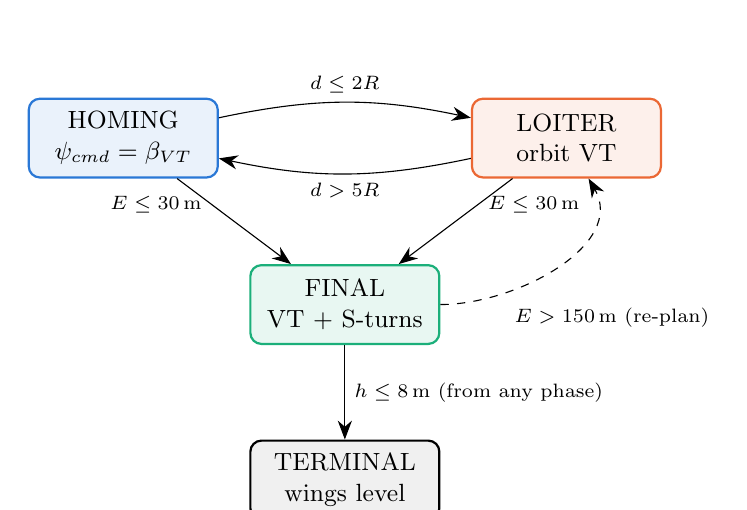
\begin{tikzpicture}[node distance=2.6cm, >={Stealth[length=2.4mm]},
  st/.style={draw, rounded corners, minimum width=2.4cm, minimum height=1cm, align=center, font=\small, thick}]
\node[st, draw=phhome, fill=phhome!10] (H) {HOMING\\$\psi_{cmd} = \beta_{VT}$};
\node[st, draw=phloit, fill=phloit!10, right=3.2cm of H] (Lo) {LOITER\\orbit VT};
\node[st, draw=phfin, fill=phfin!10, below=1.6cm of $(H)!0.5!(Lo)$] (F) {FINAL\\VT + S-turns};
\node[st, fill=lightgray, below=1.2cm of F] (T) {TERMINAL\\wings level};
\draw[->] (H) to[bend left=12] node[above, font=\scriptsize]{$d \le 2R$} (Lo);
\draw[->] (Lo) to[bend left=12] node[below, font=\scriptsize]{$d > 5R$} (H);
\draw[->] (H) -- node[pos=0.3, left, font=\scriptsize]{$E \le 30$\,m} (F);
\draw[->] (Lo) -- node[pos=0.3, right, font=\scriptsize]{$E \le 30$\,m} (F);
\draw[->, dashed] (F.east) to[out=0, in=-60] node[pos=0.25, below right=2pt, font=\scriptsize, align=left]{$E > 150$\,m (re-plan)} ([xshift=8pt]Lo.south);
\draw[->] (F) -- node[right, font=\scriptsize]{$h \le 8$\,m (from any phase)} (T);
\end{tikzpicture}
\caption{Guidance phases. From FINAL, a jump in excess energy above 150\,m
(for example after a sink-rate re-estimate) returns to LOITER if
$d \le 2R$, otherwise to HOMING.}
\end{figure}

\subsection{HOMING}
\begin{equation}
  \psi_{cmd} = \beta_{VT}, \qquad r_{ff} = 0 .
\end{equation}

\subsection{LOITER: orbit vector field}
Let $\gamma$ be the bearing from the virtual target to the canopy,
$R = \SI{50}{\meter}$ the orbit radius, $\lambda = +1$ for clockwise and
$k_o = 1.5$. The commanded heading is
\begin{equation}
  \psi_{cmd} = \gamma + \lambda\left[90^\circ + \arctan\!\left(k_o\,\frac{d - R}{R}\right)\right].
\end{equation}
On the circle ($d = R$) this is the tangent; far outside the correction tends
to $+90^\circ$ and the command points at the centre; inside it points
outward. A turn-rate feed-forward supplies the steady turn the orbit needs:
\begin{equation}
  r_{ff} = \lambda\,\frac{V_a}{R}\cdot\frac{180}{\pi}\cdot\min\!\left(1, \frac{R}{d}\right) \quad [\si{\degree\per\second}].
\end{equation}
Because the circle is centred on an air-fixed point, it is a true circle in
the air mass; over the ground it drifts downwind toward the target.

\subsection{FINAL: S-turn energy burn}
On entry the reference bearing $\psi_{ref} = \beta_{VT}$ is frozen. Flying at
an angle $\delta$ from the line of sight consumes path $L$ while closing
distance $d$ when $\cos\delta = d/L$, so
\begin{equation}
  \delta = \begin{cases} \min\!\left(\arccos\dfrac{d}{L},\ 55^\circ\right) & E > 0,\\[4pt] 0 & E \le 0 .\end{cases}
\end{equation}
The side alternates on the cross-track error from the reference line,
\begin{equation}
  x_t = (\vect p - \vect p_{VT})\cdot\begin{bmatrix}-\sin\psi_{ref}\\ \cos\psi_{ref}\end{bmatrix}
  \quad(\text{positive right of the line}),
\end{equation}
with the sign $s$ flipping from $+1$ to $-1$ when $x_t > \SI{20}{\meter}$ and
back when $x_t < -\SI{20}{\meter}$:
\begin{equation}
  \psi_{cmd} = \beta_{VT} + s\,\delta .
\end{equation}
Inside \SI{12}{\meter} of the virtual target the command is held at
$\psi_{ref}$ so the canopy never pivots over the point near the ground.

\subsection{TERMINAL}
Below $h = \SI{8}{\meter}$ steering is disabled and the servos slew to
neutral. An optional symmetric flare at \SI{3}{\meter} (both brakes pulled
350 counts) exists but is \textbf{disabled} until drop-tested.

\subsection{Loss of GPS}
If no valid fix arrives for \SI{1.5}{\second}, the last $\psi_{cmd}$ is held
on the gyro-propagated heading for a further \SI{8}{\second}. After that the
canopy flies straight (neutral servos) until GPS returns.

\subsection{Predicted miss (telemetry only)}
\begin{equation}
  \vect p_{land} = \vect p + \left(V_a\begin{bmatrix}\cos\hat\psi\\ \sin\hat\psi\end{bmatrix} + \hat{\vect W}\right)t_{go},
  \qquad \text{predMiss} = \lVert\vect p_{land}\rVert .
\end{equation}

\subsection{Guidance update in pseudocode}
\begin{algorithm}[H]
\small
\caption{\code{Guidance::update}, run at every GPS fix (\SI{5}{\hertz})}
\KwIn{$\vect p$, $h$, $V_z$, $V_a$, $\hat{\vect W}$, $\hat\psi$}
$t_{go} \leftarrow h/V_z$;\quad $\vect p_{VT} \leftarrow -\hat{\vect W} t_{go}$;\quad $\vect d \leftarrow \vect p_{VT} - \vect p$;\quad $L \leftarrow V_a t_{go}$;\quad $E \leftarrow L - \lVert\vect d\rVert$\;
\lIf{$h \le 8$}{phase $\leftarrow$ TERMINAL}
\uIf{phase = HOMING}{
  \lIf{$E \le 30$}{enter FINAL ($\psi_{ref} \leftarrow \beta_{VT}$, $s \leftarrow +1$)}
  \lElseIf{$d \le 2R$}{phase $\leftarrow$ LOITER}
}\uElseIf{phase = LOITER}{
  \lIf{$E \le 30$}{enter FINAL}
  \lElseIf{$d > 5R$}{phase $\leftarrow$ HOMING}
}\ElseIf{phase = FINAL \textbf{and} $E > 150$}{
  phase $\leftarrow$ ($d \le 2R$ ? LOITER : HOMING)\;
}
compute $\psi_{cmd}$, $r_{ff}$ for the phase (Sections 6.4 to 6.7)\;
\KwOut{$\psi_{cmd}$, $r_{ff}$, steer flag, telemetry}
\end{algorithm}

% ============================================================
\section{Inner Loop: Turn-Rate Control}
% ============================================================

\subsection{Control law}
The heading error is converted into a turn-rate command, and the gyro closes
a rate loop with feed-forward and integral action:
\begin{align}
  e &= \wrap_{180}(\psi_{cmd} - \hat\psi), \qquad e \leftarrow 0 \ \text{if}\ |e| < 2^\circ,\\
  r_{cmd} &= \sat_{\pm 22^\circ/s}\!\left(k_\psi\, e + r_{ff}\right),\\
  I &\leftarrow \sat_{\pm 250}\!\left(I + k_I\,(r_{cmd} - r)\,\Delta t\right),\\
  u^\ast &= k_{ff}\, r_{cmd} + k_r\,(r_{cmd} - r) + I,\\
  u^\ast &\leftarrow u^\ast + \operatorname{sign}(u^\ast)\, u_{slack} \quad \text{if } |u^\ast| > 1,\\
  u &\leftarrow u + \sat_{\pm 900\,\Delta t}\!\left(\sat_{\pm 450}(u^\ast) - u\right).
\end{align}
Defaults: $k_\psi = 0.6\ \si{\per\second}$, $k_{ff} = 15$ counts per
\si{\degree\per\second}, $k_r = 6$, $k_I = 8$, slack $u_{slack} = 0$ (to be
measured), slew \SI{900}{counts\per\second}. The integrator is frozen while
the output is pinned at its limit in the same direction (anti-windup) and
decays with $\tau = \SI{1}{\second}$ when steering is disabled. The loop runs
at \SI{50}{\hertz}.

\subsection{Why the earlier law $u = K_p e - K_d r$ was replaced}
An orbit requires a \emph{steady} turn rate $r_{ss} = V_a/R$, which needs a
steady brake input $u_{ss} = r_{ss}/G + u_{slack}$ where $G$ is the canopy's
turn rate per count. With $u = K_p e - K_d r$ the steady heading error is
\begin{equation}
  e_{ss} = \frac{u_{ss} + K_d\, r_{ss}}{K_p}.
\end{equation}
The damping term \emph{fights} the turn the orbit needs. Example with
$G = \SI{0.04}{\degree\per\second}$ per count, 80 counts of slack,
$r_{ss} = \SI{10}{\degree\per\second}$, $K_p = 5$, $K_d = 2.5$:
$u_{ss} = 330$ and $e_{ss} = (330 + 25)/5 = 71^\circ$. The orbit cannot be
held. The rate-command law removes the conflict: the feed-forward provides
the expected input, and the integrator absorbs unknown gain and slack. The
Monte-Carlo median miss fell from \SI{24}{\meter} to \SI{18}{\meter} when this
change was made (Table~\ref{tab:iter}).

\subsection{Brake mapping}
The canopy uses single-brake steering: only one line is pulled at a time.
\begin{equation}
  u' = \text{TURN\_SIGN}\cdot u, \qquad
  \begin{cases}
    u' > 0: & \text{right} = 2048 + s_R\,|u'|,\ \text{left} = 2048\\
    u' < 0: & \text{left} = 2048 + s_L\,|u'|,\ \text{right} = 2048
  \end{cases}
\end{equation}
with pull signs $s_L = s_R = -1$ (from the verified bench code) and positions
clamped to $[200, 3895]$. Servo 1 is the left brake. A flare pulls both by 350
counts.

% ============================================================
\section{Flight-State Machine}
% ============================================================

\begin{figure}[H]
\centering
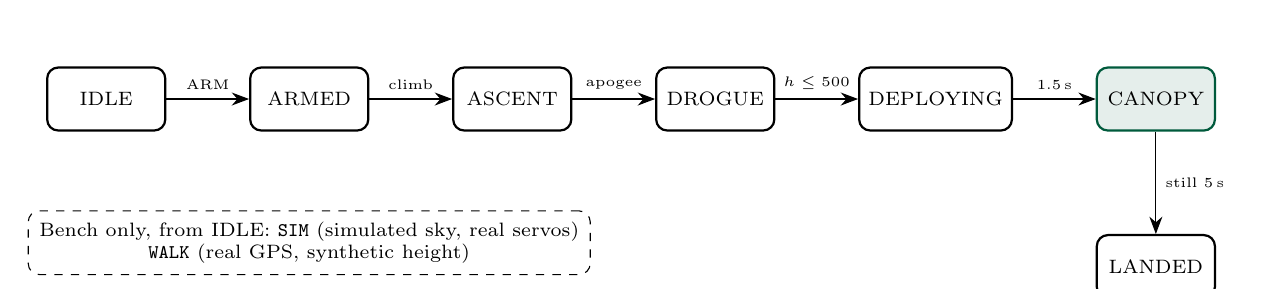
\begin{tikzpicture}[node distance=1.05cm, >={Stealth[length=2.2mm]},
  st/.style={draw, rounded corners, minimum width=1.5cm, minimum height=0.8cm, align=center, font=\scriptsize, thick}]
\node[st] (I) {IDLE};
\node[st, right=of I] (A) {ARMED};
\node[st, right=of A] (U) {ASCENT};
\node[st, right=of U] (D) {DROGUE};
\node[st, right=of D] (P) {DEPLOYING};
\node[st, right=of P, fill=isrogreen!10, draw=isrogreen] (C) {CANOPY};
\node[st, below=1.3cm of C] (L) {LANDED};
\draw[->] (I) -- node[above, font=\tiny]{ARM} (A);
\draw[->] (A) -- node[above, font=\tiny]{climb} (U);
\draw[->] (U) -- node[above, font=\tiny]{apogee} (D);
\draw[->] (D) -- node[above, font=\tiny]{$h\le500$} (P);
\draw[->] (P) -- node[above, font=\tiny]{1.5\,s} (C);
\draw[->] (C) -- node[right, font=\tiny]{still 5\,s} (L);
\node[below=1.0cm of A, font=\scriptsize, align=center, draw, dashed, rounded corners, inner sep=4pt]
  (B) {Bench only, from IDLE: \code{SIM} (simulated sky, real servos)\\ \code{WALK} (real GPS, synthetic height)};
\end{tikzpicture}
\caption{Flight-state machine in the \code{.ino}. Inside CANOPY the
\code{FlightCore} runs DAMPING (8\,s) $\to$ GUIDED $\to$ TERMINAL.}
\end{figure}

\begin{center}
\small
\renewcommand{\arraystretch}{1.2}
\begin{tabularx}{\linewidth}{p{3.2cm}Y}
\toprule
\rowcolor{tblhead}\hdr{Transition} & \hdr{Condition} \\
\midrule
IDLE $\to$ ARMED & \code{ARM} command; both servos answer; baro or GPS altitude available. Captures $p_0$, gyro bias, GPS ground altitude; locks the SG90 at \SI{140}{\degree}; opens the log. \\
ARMED $\to$ ASCENT & $h > \SI{30}{\meter}$ and $\hat v > \SI{8}{\meter\per\second}$ up \\
ASCENT $\to$ DROGUE & $\hat v < -\SI{2}{\meter\per\second}$ for \SI{1}{\second}, or $h < h_{max} - \SI{15}{\meter}$ \\
DROGUE $\to$ DEPLOYING & $h \le \SI{500}{\meter}$ while descending; or, if $h_{max} < \SI{520}{\meter}$, \SI{2}{\second} after apogee. SG90 to \SI{180}{\degree}. \\
DEPLOYING $\to$ CANOPY & after \SI{1.5}{\second}; \code{FlightCore.startDescent()} \\
CANOPY $\to$ LANDED & $h < \SI{20}{\meter}$, $|\hat v| < \SI{0.4}{\meter\per\second}$, ground speed $< \SI{1}{\meter\per\second}$ for \SI{5}{\second}; or \SI{900}{\second} timeout \\
\bottomrule
\end{tabularx}
\end{center}

\paragraph{Reset recovery.} On entering ARMED, ASCENT, DROGUE, DEPLOYING or
CANOPY the firmware writes a \code{ResumeRecord} (state, $p_0$, target,
elevation offset, GPS ground altitude) to EEPROM, protected by an FNV-1a
checksum. After a watchdog reset in flight it resumes: from DEPLOYING or
CANOPY directly into guided flight, from ASCENT or DROGUE into DROGUE. The
record is cleared on LANDED, IDLE or \code{CLEAR}.

% ============================================================
\section{Firmware Implementation}
% ============================================================

\subsection{Scheduling}
The main loop is fully non-blocking apart from short servo-bus pauses.
\begin{center}
\small
\begin{tabular}{lrl}
\toprule
\textbf{Task} & \textbf{Rate} & \textbf{Notes} \\
\midrule
GPS parse & every loop & one update per epoch (RMC trigger) \\
IMU yaw rate & \SI{100}{\hertz} & heading propagation \\
Barometer & \SI{25}{\hertz} & alpha-beta filter \\
Compass & \SI{10}{\hertz} & fallback heading \\
Control (\code{FlightCore.step}) & \SI{50}{\hertz} & inner loop \\
Servo write & \SI{20}{\hertz} max & only on change $\ge 4$ counts \\
USB telemetry \code{GUIDE} & \SI{4}{\hertz} & switchable with \code{TLM} \\
SD log & \SI{10}{\hertz} & flushed every \SI{1}{\second} \\
\bottomrule
\end{tabular}
\end{center}

\subsection{GPS configuration and quality gate}
At boot a UBX-CFG-VALSET message (class 0x06, ID 0x8A, RAM layer) is sent:
\begin{center}
\small
\begin{tabular}{llll}
\toprule
\textbf{Key} & \textbf{ID} & \textbf{Value} & \textbf{Verified} \\
\midrule
CFG-RATE-MEAS & 0x30210001 & \SI{200}{\milli\second} (\SI{5}{\hertz}) & \good{yes, 5.0\,Hz measured} \\
CFG-NAVSPG-DYNMODEL & 0x20110021 & 6 (airborne $<$1\,g) & \warn{not checked} \\
NMEA GSV / GLL / VTG on UART1 & 0x209100C5 / CA / B1 & 0 (off) & \warn{not checked} \\
\bottomrule
\end{tabular}
\end{center}
A fix is accepted when it is valid, younger than \SI{1500}{\milli\second},
uses at least 5 satellites and has HDOP $\le 4.0$ (\code{FLIGHT}) or
$\le 8.0$ (\code{LAB}). The earlier code's fixed limit of 3.5 had blocked all
steering at HDOP 5.13 indoors.

\subsection{BMP581 register driver}
Soft reset (0xB6 to 0x7E), chip ID check (0x50, or 0x51 for BMP585), NVM
status check and standby. Then OSR\_CONFIG (0x36) is set to 0x58: pressure
enabled, $8\times$ pressure and $1\times$ temperature oversampling. ODR\_CONFIG (0x37) is set to 0xBD: normal mode, \SI{50}{\hertz}, deep standby
disabled. Six bytes from
0x1D give
\begin{equation}
  T = \frac{\text{raw}_{24,\text{signed}}}{65536}\ [\si{\celsius}], \qquad
  p = \frac{\text{raw}_{24}}{64}\ [\si{\pascal}],
\end{equation}
with a sanity window \SIrange{30}{115}{\kilo\pascal}.

\subsection{Other sensors}
\begin{itemize}
  \item \textbf{QMC5883:} 0x0B $\leftarrow$ 0x01, 0x09 $\leftarrow$ 0x1D;
        calibrated $(x,y)$ with offsets (180, 336) and scales
        (0.9565, 0.9044); navigation heading mirrored, $360^\circ -
        \operatorname{atan2}(y,x)$, as found in the earlier compass test.
  \item \textbf{LSM6DSO32} (Adafruit LSM6DSOX driver): $\pm16$\,g,
        $\pm\SI{2000}{\degree\per\second}$, \SI{208}{\hertz}. Yaw rate =
        $-\omega_z$ (Z axis up). Bias averaged over 200 samples at boot and
        at ARM.
\end{itemize}

\subsection{ST-3009 servo bus}
SCServo \code{SMS\_STS} on Serial1 half-duplex at \SI{1}{Mbps}.
\code{WritePosEx(id, pos, 500, 50)}: speed 500 and acceleration 50 match the
team's working stand-alone test. Each write checks the servo's
acknowledgement; a missing ACK leaves the position unmarked so it is resent
on the next \SI{50}{\milli\second} cycle. Torque is enabled explicitly at
boot. A background PING every \SI{2}{\second} tracks bus health.

\subsection{Command interface}
\begin{center}
\small
\renewcommand{\arraystretch}{1.12}
\begin{tabularx}{\linewidth}{p{4.3cm}Y}
\toprule
\rowcolor{tblhead}\hdr{Command} & \hdr{Action} \\
\midrule
\code{HELP}, \code{STATUS} & command list; full system status \\
\code{ARM}, \code{DISARM}/\code{STOP}, \code{CLEAR} & arm for flight; return to IDLE; erase resume record \\
\code{TARGET lat lon}, \code{TARGETHERE}, \code{ELEV m} & set target; target = current fix; target elevation offset \\
\code{DEPLOY}, \code{PREP} & SG90 release; SG90 lock \\
\code{CENTER}, \code{LEFT [n]}, \code{RIGHT [n]}, \code{MOTORTEST} & manual steering in IDLE \\
\code{PING}, \code{TORQUE}, \code{SPEED n}, \code{BUSTEST} & servo diagnostics (position, supply, temperature, missed ACKs) \\
\code{HEALTH ON|OFF}, \code{SERVODBG ON|OFF} & background PING; print every servo write \\
\code{SIM [n e h wN wE]} & simulated descent driving the real servos \\
\code{WALK} & walking test with real GPS, synthetic height \\
\code{GAINS kPsi kR kI kFF}, \code{SLACK n}, \code{LOITER R dir} & runtime tuning \\
\code{LAB}, \code{FLIGHT} & HDOP gate 8.0 or 4.0 \\
\code{GYROTEST}, \code{BARO}, \code{LOG ON|OFF}, \code{TLM ON|OFF} & sensor checks, logging, telemetry \\
\bottomrule
\end{tabularx}
\end{center}

\subsection{Telemetry record}
Each \code{GUIDE} line (USB and SD) contains: time, flight state, core mode,
phase, latitude, longitude, $p_N$, $p_E$, $h$, $V_z$, ground speed,
$\hat\psi$, $\psi_{cmd}$, $r_{cmd}$, $r$, demand $u$, servo 1 and 2 positions,
$\hat W_N$, $\hat W_E$, wind-valid flag, $V_a$, $t_{go}$, $L$, $d$, $E$,
$\vect p_{VT}$, predicted miss, satellites, HDOP and GPS-OK flag. This record
contains everything needed to measure the canopy's airspeed, sink rate and
turn response after a drop test.

% ============================================================
\section{Monte-Carlo Verification}
% ============================================================

\subsection{Method}
The harness \code{host\_sim/monte\_carlo.cpp} runs complete descents through
the \emph{same} \code{FlightCore} object the Teensy runs. The controller is
given only the defaults ($V_a = 6$, $V_z = \SI{2.5}{\meter\per\second}$) and
must measure everything else, as in flight.

\subsection{Vehicle model}
Brake slack $u_0$ is removed, the steady turn rate follows with a first-order
lag, and turning increases sink:
\begin{align}
  u_{eff} &= \operatorname{sign}(u)\max(|u| - u_0, 0), \qquad
  r_{ss} = \sat_{\pm r_{max}}\!\left(G\,\rho\, u_{eff}\right),\\
  \dot r &= \frac{r_{ss} - r}{\tau}, \qquad \dot\psi = r, \qquad
  V_z = V_{z0}\left[1 + \kappa\left(\frac{r}{r_{max}}\right)^{2}\right],\\
  \dot{\vect p} &= V_a\begin{bmatrix}\cos\psi\\ \sin\psi\end{bmatrix} + \vect W(h) + \vect g(t),
  \qquad \dot h = -V_z,
\end{align}
where $\rho$ is the right/left gain ratio for right turns. Wind follows a
power-law shear with directional veer, and gusts are a first-order
Gauss-Markov process:
\begin{align}
  \vect W(h) &= \left(\frac{h}{500}\right)^{\alpha} \mathbf{R}\!\left(\theta_v\left(1 - \tfrac{h}{500}\right)\right)\vect W_{500},\\
  d\vect g &= -\frac{\vect g}{\tau_g}\,dt + \sigma_g\sqrt{\frac{2\,dt}{\tau_g}}\;\vect n, \qquad \vect n \sim \mathcal N(0, I),\ \tau_g = \SI{4}{\second}.
\end{align}

\subsection{Randomised parameters}
\begin{center}
\small
\renewcommand{\arraystretch}{1.15}
\begin{tabularx}{\linewidth}{p{4.2cm}Yp{3.0cm}}
\toprule
\textbf{Quantity} & \textbf{Distribution} & \textbf{Purpose} \\
\midrule
Airspeed $V_a$ & $\mathcal U(5, 8)$\,\si{\meter\per\second} & unknown canopy \\
Sink $V_{z0}$ & $\mathcal U(1.8, 3.5)$\,\si{\meter\per\second} & unknown canopy \\
Turn gain $G$ & $\mathcal U(0.035, 0.09)$\,\si{\degree\per\second} per count & unknown linkage \\
Right/left ratio $\rho$ & $\mathcal U(0.8, 1.25)$ & asymmetric rigging \\
Turn lag $\tau$ & $\mathcal U(0.3, 1.2)$\,\si{\second} & canopy inertia, pendulum \\
Brake slack $u_0$ & $\mathcal U(0, 80)$ counts & line slack \\
Max turn rate & $\mathcal U(25, 45)$\,\si{\degree\per\second} & \\
Turn sink factor $\kappa$ & $\mathcal U(0.2, 0.8)$ & \\
Wind at \SI{500}{\meter} & $\mathcal U(0, 6)$\,\si{\meter\per\second}, any direction & \\
Shear exponent $\alpha$, veer $\theta_v$ & $\mathcal U(0.08, 0.25)$, $\mathcal U(-25^\circ, 25^\circ)$ & \\
Gust $\sigma_g$ & $\mathcal U(0.2, 1.0)$\,\si{\meter\per\second} & \\
Deployment height & $\mathcal U(470, 530)$\,\si{\meter} & \\
Deployment distance & $\mathcal U(0, 900)$\,\si{\meter}, any bearing & rocket drift \\
GPS & \SI{5}{\hertz}, \SI{0.15}{\second} latency, \SI{0.8}{\meter} white + random-walk position, \SI{0.15}{\meter\per\second} velocity & \\
GPS dropout & 20\,\% of flights, \SI{10}{\second} at a random time in \SIrange{20}{120}{\second} & \\
Baro & \SI{25}{\hertz}, \SI{0.25}{\meter} noise, ground bias $\mathcal U(\pm3)$\,\si{\meter} & \\
Gyro & \SI{0.5}{\degree\per\second} noise, residual bias $\mathcal U(\pm0.6)$\,\si{\degree\per\second} & \\
\bottomrule
\end{tabularx}
\end{center}
Each flight uses its own random seed, so code changes are compared on
identical flights.

\subsection{Reachability classification}
Using the true parameters, the reach margin at deployment is
\begin{equation}
  M = V_a\, t_{av} - \bigl\lVert \vect p_0 + \bar{\vect W}\, t_{av} \bigr\rVert,
  \qquad t_{av} = \frac{h_0 - V_{z0}\,T_{damp}}{V_{z0}},
\end{equation}
with $\bar{\vect W}$ the wind averaged over the descent. $M < 0$: physically
unreachable. $0 \le M \le \SI{150}{\meter}$: marginal. $M > \SI{150}{\meter}$:
comfortable.

\subsection{Results}
\begin{table}[H]
\centering
\small
\renewcommand{\arraystretch}{1.2}
\begin{tabular}{lrcccc}
\toprule
\rowcolor{tblhead}\hdr{Class (seed 99, 3000 flights)} & \hdr{N} & \hdr{$\le$80\,m} & \hdr{Median} & \hdr{95th pct.} \\
\midrule
All flights (incl.\ unreachable) & 3000 & 89.1\,\% & \SI{15.6}{\meter} & \SI{289}{\meter} \\
Reachable ($M \ge 0$) & 2684 & \good{98.3\,\%} & \SI{14}{\meter} & n/a \\
\quad Marginal ($0 \le M \le 150$\,m) & 233 & 82.4\,\% & \SI{22.4}{\meter} & n/a \\
\quad Comfortable ($M > 150$\,m) & 2451 & \good{99.8\,\%} & \SI{13.9}{\meter} & \SI{34.4}{\meter} \\
Wind $\ge$ \SI{4}{\meter\per\second} (all) & 1007 & n/a & \SI{22.6}{\meter} & n/a \\
GPS-dropout flights (all) & 603 & n/a & \SI{15.3}{\meter} & n/a \\
\bottomrule
\end{tabular}
\caption{Final configuration. Almost every miss above 80\,m is a flight
whose target was outside, or at the edge of, the canopy's physical reach.}
\end{table}

\begin{table}[H]
\centering
\small
\renewcommand{\arraystretch}{1.2}
\begin{tabular}{lccc}
\toprule
\textbf{Configuration} & \textbf{Reachable $\le$80\,m} & \textbf{Comfortable $\le$80\,m} & \textbf{Comfortable median / 95th} \\
\midrule
New, GPS \SI{5}{\hertz} (seed 99) & 98.3\,\% & 99.8\,\% & 13.9 / 34.4\,m \\
New, GPS \SI{1}{\hertz} (seed 99) & 97.9\,\% & 99.5\,\% & 14.9 / 37.7\,m \\
New, independent seed 123 & 98.2\,\% & 99.8\,\% & 13.7 / 32.5\,m \\
Old point-at-target logic (seed 99) & 97.2\,\% & 98.9\,\% & 29.4 / 61.8\,m \\
\bottomrule
\end{tabular}
\caption{Comparisons. The old logic was emulated with loiter, final and wind
compensation disabled (pure bearing pursuit, no 35\,m capture).}
\end{table}

\begin{figure}[H]
\centering
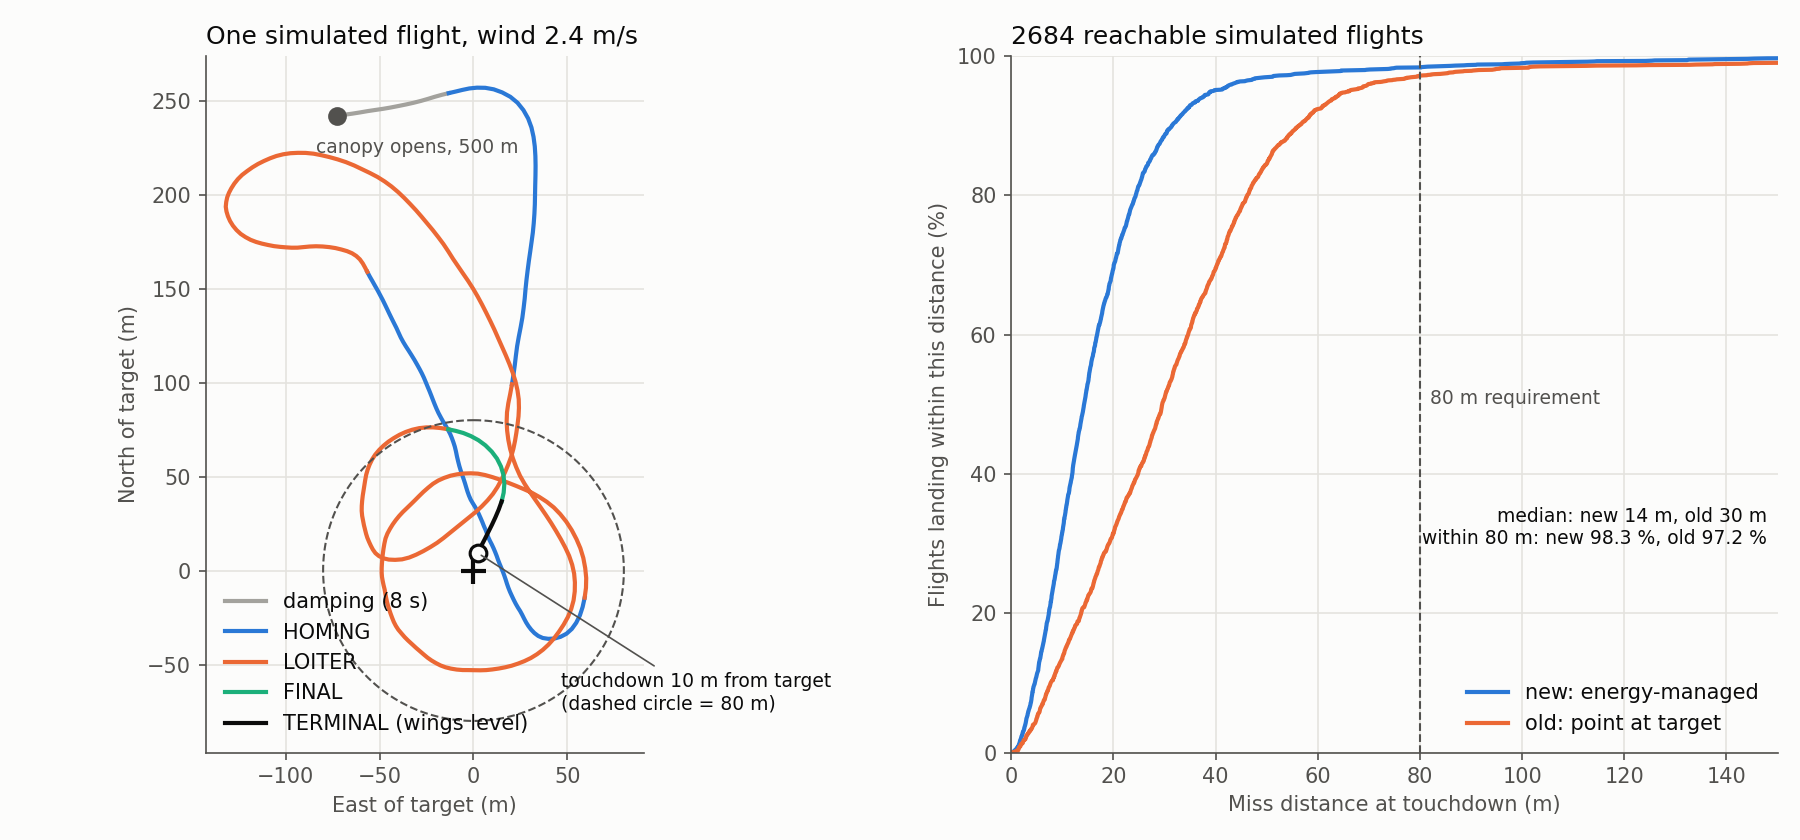
\includegraphics[width=\linewidth]{guidance_results.png}
\caption{Left: one simulated flight through all phases (wind 2.4\,m/s,
touchdown 10\,m from the target); the loiter circles drift downwind with the
air mass. Right: cumulative miss distance over the reachable flights, new
versus old logic.}
\end{figure}

\paragraph{An honest note on the old logic.} Without its 35\,m capture
rule, pure pursuit already lands within 80\,m in 97\,\% of reachable cases in
this model, because overflying the target makes it spiral tightly overhead.
The new law halves the median and 95th-percentile miss, but its larger
real-world advantage is not captured by the model: it flies gentle
\SI{50}{\meter} orbits at about \SI{8}{\degree\per\second} and keeps the wings
level near the ground, whereas pursuit spirals at full brake for minutes,
which on a real canopy risks a spiral dive, high sink and pendulum coupling.

\subsection{Design iterations driven by the simulation}
\begin{table}[H]
\centering
\small
\renewcommand{\arraystretch}{1.2}
\begin{tabularx}{\linewidth}{p{6.2cm}ccY}
\toprule
\textbf{Version (seed 1, 1000 paired flights)} & \textbf{Reachable $\le$80\,m} & \textbf{Comfortable $\le$80\,m} & \textbf{Comfortable median / 95th} \\
\midrule
v1: open-loop wind-ID turn, $u = K_p e - K_d r$ & 92.5\,\% & 97.2\,\% & 23.8 / 58.9\,m \\
v2: wind-fit coverage from gyro heading & 92.0\,\% & 97.7\,\% & 23.7 / 54.5\,m \\
v3: turn-rate inner loop + orbit feed-forward & 93.1\,\% & 98.5\,\% & 18.0 / 40.8\,m \\
v4: skip wind-ID turn when energy is tight & 96.0\,\% & 98.7\,\% & 18.0 / 40.4\,m \\
\bottomrule
\end{tabularx}
\caption{Iteration history. v1 was run before per-flight seeding was added, so its flights are a different random draw; v2 to v4 are paired. v5 ($R = 50$\,m, exit margin 30\,m) and v6
(wind-ID turn removed) were evaluated on seed 99, Table~\ref{tab:idturn}.}
\label{tab:iter}
\end{table}

\begin{table}[H]
\centering
\small
\renewcommand{\arraystretch}{1.2}
\begin{tabular}{lcc}
\toprule
\textbf{Wind-ID turn policy (seed 99, 3000 flights)} & \textbf{Marginal $\le$80\,m} & \textbf{Comfortable $\le$80\,m} \\
\midrule
ID turn if reach margin $>$ 300\,m & 50.6\,\% & 99.1\,\% \\
ID turn if reach margin $>$ 500\,m & 64.4\,\% & 99.3\,\% \\
ID turn if reach margin $>$ 800\,m & 77.3\,\% & 99.6\,\% \\
\textbf{No dedicated ID turn (final)} & \good{82.4\,\%} & \good{99.8\,\%} \\
\bottomrule
\end{tabular}
\caption{A dedicated 330$^\circ$ wind-identification turn after damping
always cost more altitude than it returned. The loiter turns measure the
wind for free, so the ID turn is disabled by default.}
\label{tab:idturn}
\end{table}

\subsection{Sensitivity (seed 99, 1500 flights, comfortable class)}
\begin{center}
\small
\renewcommand{\arraystretch}{1.15}
\begin{tabular}{lccc}
\toprule
\textbf{Variation} & \textbf{$\le$80\,m} & \textbf{Median} & \textbf{95th pct.} \\
\midrule
Baseline (baro ground bias $\pm$3\,m) & 99.8\,\% & 13.9\,m & 35.3\,m \\
Baro / target-elevation bias $\pm$10\,m & 99.7\,\% & 18.8\,m & 45.0\,m \\
Baro / target-elevation bias $\pm$20\,m & \warn{98.6\,\%} & 27.2\,m & \warn{63.7\,m} \\
\midrule
Gains $k_\psi, k_r, k_I$ = 0.3, 2, 3 & 99.7\,\% & 16.5\,m & 43.9\,m \\
Gains = 0.4, 3, 4 & 99.8\,\% & 14.9\,m & 38.9\,m \\
Gains = 0.6, 6, 8 (default) & 99.8\,\% & 13.9\,m & 35.3\,m \\
Gains = 0.8, 8, 10 & 99.8\,\% & 13.4\,m & 33.6\,m \\
\midrule
$R$ = 35\,m, exit margin 30\,m & 99.8\,\% & 14.9\,m & 38.7\,m \\
$R$ = 70\,m, exit margin 30\,m & 99.8\,\% & 15.2\,m & 36.8\,m \\
$R$ = 50\,m, exit margin 15 / 45 / 60\,m & 99.8\,\% & 16.6 / 17.9 / 20.7\,m & 40.8 / 36.7 / 41.8\,m \\
\bottomrule
\end{tabular}
\end{center}
The design is robust to gains and orbit size. The dominant external error is
\textbf{height reference}: a wrong target-ground elevation directly scales
$t_{go}$. The target elevation relative to the ARM point must be known within
a few metres (\code{ELEV} command).

% ============================================================
\section{Hardware Bench and Ground Tests}
% ============================================================

\begin{center}
\small
\renewcommand{\arraystretch}{1.22}
\begin{tabularx}{\linewidth}{p{2.6cm}Yp{1.6cm}}
\toprule
\rowcolor{tblhead}\hdr{Test} & \hdr{Result} & \hdr{Verdict} \\
\midrule
1.\ Compile and boot & IMU, BMP581 (chip 0x50), QMC5883 and both ST-3009 detected; gyro bias \SI{0.32}{\degree\per\second}. SD and watchdog not yet installed. & \good{pass} \\
2.\ Steering servos & PING OK, positions 2048/2047, supply 7.6 and \SI{7.7}{\volt}. \code{LEFT} moves only ID 1, \code{RIGHT} only ID 2. & \good{pass} \\
3.\ Gyro direction and scale & Clockwise rotation increases heading; a measured \SI{180}{\degree} turn read \SI{180}{\degree}. & \good{pass} \\
4.\ Barometer & $p$ = 94\,938\,Pa, $T$ = \SI{22}{\celsius}; noise about $\pm$\SI{0.15}{\meter} at rest; lift read +\SI{0.6}{\meter} (7.5\,Pa) and returned to zero. & \good{pass} \\
5.\ SIM descent on real servos & \code{SIM 400 300 500 2 1}: full phase sequence, no missed ACKs, touchdown \SI{13.9}{\meter} from target. & \good{pass} \\
6.\ GPS outdoors & 12 satellites, HDOP 0.70, \SI{5.0}{\hertz} after the epoch fix. & \good{pass} \\
7.\ WALK test & Correct servo indicates turn toward the target; LOITER engaged within \SI{100}{\meter}; GPS 5.0\,Hz, HDOP 0.48. & \good{pass} \\
8.\ SD log and watchdog & pending & \warn{open} \\
\bottomrule
\end{tabularx}
\end{center}

\subsection{Defects found and fixed during bench testing}
\begin{enumerate}
  \item \textbf{Compile error ``\code{ResumeRecord} does not name a type''.}
        The Arduino IDE inserts function prototypes before the first function
        in the \code{.ino}, ahead of the struct. Fixed by moving the struct
        into \code{ResumeRecord.h}.
  \item \textbf{Servos commanded but not moving, Servo 1 vibrating.} The team's
        stand-alone test moved both servos. Changes made: speed 2400 to 500
        (matching the working test), explicit torque enable, and ACK checking
        with automatic resend. After these changes both servos respond
        correctly. \emph{The single root cause was not isolated}; the ACK
        counter in \code{PING} should be watched in further tests.
  \item \textbf{GPS rate reported as \SI{10}{\hertz}.} Each epoch produced two
        updates (GGA and RMC both carry position), so every fix was also fed
        to guidance twice. Fixed by triggering once per epoch on RMC.
\end{enumerate}

% ============================================================
\section{Limitations and Open Items}
\label{sec:limits}
% ============================================================

\begin{itemize}
  \item \textbf{Not yet flown or drop-tested.} Airspeed, sink rate, turn rate
        per count, lag and brake slack are modelling ranges. The Monte-Carlo
        results hold only if the real canopy lies inside those ranges.
  \item \textbf{Physical reach governs the requirement.} With
        $V_a = 6$ and $V_z = \SI{2.5}{\meter\per\second}$ the still-air reach
        from \SI{500}{\meter} is about \SI{1.1}{\kilo\meter} after damping, less
        into a headwind. The deployment point relative to the target matters
        as much as the software.
  \item \textbf{Steering sign with the canopy attached.} \code{TURN\_SIGN} and
        the pull signs are set from bench rotation only; a reversed sign
        would steer away from the target. It must be confirmed in the first
        drop.
  \item \textbf{Brake slack} (\code{SLACK}) is zero until measured.
  \item \textbf{Height reference.} \code{TARGET\_ELEV\_OFFSET\_M} must be
        known within a few metres.
  \item \textbf{GPS settings} other than the measurement rate (dynamic model,
        NMEA trimming) are sent but not confirmed.
  \item \textbf{Flare} is disabled until tested.
  \item \textbf{Watchdog and SD logging} are not yet installed on the bench
        unit.
  \item \textbf{Model simplifications:} no pendulum dynamics, no canopy
        collapse, terrain assumed flat at target elevation.
\end{itemize}

% ============================================================
\section{Next Steps}
% ============================================================
\begin{enumerate}
  \item Install the WDT\_T4 library and a FAT32 microSD; verify \code{FLT000.CSV}.
  \item \textbf{Drop test 1, steering sign:} \code{LEFT}/\code{RIGHT} fixed
        demands in turn, confirm the canopy turns in the commanded direction.
  \item \textbf{Characterisation drops:} straight segments for $V_a$, $V_z$
        and glide ratio; step demands of 100 to 450 counts for turn gain $G$,
        lag $\tau$ and slack $u_0$, all from the \code{GUIDE} log.
  \item Set \code{SLACK}, re-run the Monte-Carlo with the measured
        parameters narrowed in, and retune \code{GAINS} if needed.
  \item Guided drops from increasing heights with a ground target; compare
        touchdown with the logged predicted miss.
  \item Confirm the expected deployment point from the rocket trajectory lies
        well inside the canopy's reach envelope.
\end{enumerate}

% ============================================================
\appendix
\section{Default Parameters}
% ============================================================
\begin{center}
\small
\renewcommand{\arraystretch}{1.1}
\begin{longtable}{lll}
\toprule
\textbf{Parameter} & \textbf{Value} & \textbf{Where} \\
\midrule
\endhead
Loiter radius $R$, direction & 50\,m, clockwise & \code{GuidanceConfig} \\
Orbit gain $k_o$ & 1.5 & \\
Loiter entry / leave & $d \le 2R$ / $d > 5R$ & \\
Final exit margin & 30\,m & \\
Final return-to-loiter & $E > 150$\,m & \\
S-turn max angle / cross-track limit & 55$^\circ$ / 20\,m & \\
Final no-turn distance & 12\,m & \\
Terminal height & 8\,m & \\
Clamps: wind, $V_z$, $V_a$ & 12\,m/s; 0.8 to 8\,m/s; 2.5 to 15\,m/s & \\
\midrule
$k_\psi$, $r_{cmd,max}$ & 0.6\,s$^{-1}$, 22\,$^\circ$/s & \code{SteeringConfig} \\
$k_{ff}$, $k_r$, $k_I$, $I_{max}$ & 15, 6, 8, 250 counts & \\
Heading deadband, max demand, slew & 2$^\circ$, 450 counts, 900 counts/s & \\
\midrule
Damping time & 8\,s & \code{CoreConfig} \\
Wind-ID turn & disabled & \\
GPS timeout / heading hold & 1.5\,s / 8\,s & \\
Heading GPS gain, latency comp. & 0.30, 0.15\,s & \\
Min speed for GPS heading & 1.5\,m/s (0.6 in WALK) & \\
Compass fallback gain & 0.05 & \\
Default $V_a$, $V_z$ & 6, 2.5\,m/s & \\
Straight-flight threshold & $|r| < 6^\circ$/s for 2\,s & \\
$\tau_z$, $\tau_{V_a}$ & 3\,s, 4\,s & \\
Alpha-beta $\alpha$, $\beta$ & 0.12, 0.008 & \\
Wind window, solve period & 160 samples, 1\,s & \\
\midrule
Parafoil deploy height & 500\,m & \code{.ino} \\
Launch detect & $h > 30$\,m, $\hat v > 8$\,m/s & \\
Apogee & $\hat v < -2$\,m/s for 1\,s or 15\,m drop & \\
Landed & $h < 20$\,m, still 5\,s & \\
GPS gate & $\ge$5 sats, HDOP $\le$4 (8 in LAB), age $<$1.5\,s & \\
Servo speed / accel & 500 / 50 & \\
Servo neutral / range & 2048 / 200 to 3895 & \\
Pull signs, \code{TURN\_SIGN} & $-1$, $-1$, $+1$ (verify with canopy) & \\
\bottomrule
\end{longtable}
\end{center}

% ============================================================
\section{Reproducing the Monte-Carlo Results}
% ============================================================
\begin{verbatim}
cd Parafoil_Guided_Landing/host_sim
g++ -O2 -std=c++14 -o mc monte_carlo.cpp
./mc 3000 5 99            # final configuration, 5 Hz GPS
./mc 3000 1 99            # same flights, 1 Hz GPS
MC_OLD=1 ./mc 3000 5 99   # emulate the old point-at-target logic
MC_BARO=20 ./mc 1500 5 99 # +/-20 m height-reference error
MC_R=70 MC_EXTRA=30 ./mc 1500 5 99   # orbit radius / exit margin
MC_KPSI=0.8 MC_KR=8 MC_KI=10 ./mc 1500 5 99   # inner-loop gains
MC_IDMARGIN=300 ./mc 3000 5 99       # re-enable wind-ID turn
MC_FAIL=1 ./mc 1000 5 1   # print every flight that misses by > 80 m
\end{verbatim}

\end{document}
